\chapter{Modelización de la tarea de aprendizaje} \label{ch:tarea_aprendizaje}

\section{Planteamiento del problema} \label{seq:planteamiento_problema}

La tarea de aprendizaje que consideramos es la de clasificación. Durante todo el desarrollo, pensaremos en la \textbf{clasificación de imágenes}. En este caso, el enfoque que más éxito ha tenido históricamente es el uso de redes convolucionales profundas y, más actualmente, el uso del modelo \entrecomillado{transformer}.

Dado un elemento $X = (\nv{x_1}, \ldots, \nv{x_N})$, donde $\nv{x_i} \in \R^s \ \forall i \in \deltaset{N}$, queremos clasificarlo en alguna de las etiquetas $\mathcal{Y} = \{1, \ldots, Y \} = \deltaset{Y}$.

Con esto, podemos ver que los datos de entrada viven en el espacio

$$\mathcal{X} := \R^s \times \overset{N}{\ldots} \times \R^s = (\R^s)^N$$

Esta representación de los datos de entrada es natural en muchas situaciones. En el caso de las imágenes, podemos considerar cada vector $\nv{x_i}$ como un conjunto de \textit{pixels} de la imagen. Idealmente, cada vector de \textit{pixels} debería contener un vecindario de \textit{pixels}, es decir, \textit{pixels} adyacentes. Podemos incluso considerar \textit{pixels} que aparezcan en más de un vector. Por ejemplo, podemos considerar $\nv{x_i}$ como la fila o columna $i$-ésima de la imagen.

Por ejemplo, el trabajo que presenta el conocido modelo  de deep learning \textit{VIT} propone una arquitectura \entrecomillado{transformer} a la que que se le pasa \entrecomillado{patches} de la imagen para poder explotar el mecanismo de atención: \entrecomillado{we split an image into patches and provide the sequence of linear embeddings of these patches as an input to a Transformer} \footnote{\cite{matematicas:vit}}
\todo{No sé si así está bien referenciado el trabajo al que me refiero}

Para decidir la etiqueta de un elemento, consideramos $Y$ \textbf{funciones de puntuación}:

$$\{h_y: \mathcal{X} \to \R \dspace / \dspace y \in \mathcal{Y} \}$$

Con esto, dado un elemento $X \in \mathcal{X}$, lo clasificaremos buscando la etiqueta cuya función de puntuación sea máxima, es decir:

$$\hat{y} := \underset{y \in \mathcal{Y}}{argmax} \dspace h_y(X)$$

Por tanto, nuestro \textbf{espacio de hipótesis} $\Gamma$ es el conjunto de funciones $\mathcal{X} \to \R$. Tanto en la práctica con modelos de \textit{machine learning}, como en nuestras dos modelizaciones, trabajamos en un subconjunto $\tilde{\Gamma} \subseteq \Gamma$ de funciones de puntuación, implementables o bien por el modelo de \textit{machine learning} o bien por nuestra modelización teórica.

\section{Espacio de hipótesis general}

Nuestro objetivo en esta sección es justificar la elección de las funciones $h_y$ en \customref{sec:repr_funciones_puntuacion}, que conformarán el espacio de hipótesis sobre el que trabajaremos.

\subsection{Preliminares sobre los espacios $L^2$} \label{sec:preliminares_funcional}

A continuación, introduciremos algunos conceptos sobre espacios de funciones que serán fundamentales en la justificación de la elección de las funciones $h_y$. Empezamos introduciendo el siguiente espacio de funciones, que es de sobra conocido:

\begin{definicion}[Espacio de Lebesgue]

    Dado $\Omega \subseteq \R^N$ definimos el siguiente espacio de funciones:

    \begin{equation}
        \mathcal{L}(\Omega) := \{f: \Omega \to \R : f \dspace \text{es medible} \}
    \end{equation}

    Sobre dicho espacio, definimos la siguiente relación de equivalencia:

    \begin{equation}
        f \sim g \iff f = g \dspace \text{cpd en } \Omega
    \end{equation}

    Y con ello definimos el \textbf{espacio de Lebesgue sobre $\Omega$} como:

    \begin{equation}
        L(\Omega) := \mathcal{L} / \sim
    \end{equation}
\end{definicion}

Y ahora, introducimos el siguiente espacio de funciones:

\begin{definicion}[Espacios de Lebesgue $L^p$]
    Dado $\Omega \subseteq \R^N$ definimos

    \begin{equation}
        \mathcal{L}^p := \{ f \in \mathcal{L} : \int_{\Omega} |f|^p d\mu < \infty \}
    \end{equation}

    y, como hemos hecho previamente, definimos:

    \begin{equation}
        L^p(\Omega) := \mathcal{L}^p / \sim
    \end{equation}

\end{definicion}
\todo{\textbf{CUIDADO} Revisar que esto es correcto porque lo estoy haciendo de cabeza mientras escribo el Latex}

A partir de estas definiciones, nos centraremos en los espacios $L^2(\R^N)$, escribiendo $L^2$ cuando esto no de lugar a confusión. Sabemos de sobra que este espacio es de Hilbert, considerando el producto escalar:

\begin{equation}
    \innerproduct{f}{g} := \int_{\Omega} f \cdot g d\mu
\end{equation}

Además, usaremos el siguiente hecho:

\begin{proposicion}
    En un espacio vectorial $\mathbb{V}$ de \textit{Hilbert} de dimensión finita, donde tenemos una base vectorial, convergencia en norma implica convergencia en los coeficientes en dicha base
\end{proposicion}

\begin{proof}
    Disponemos de una base vectorial $\mathbb{B} = \conjunto{e_1, \ldots, e_N}$. Además, por el método de Gram–Schmidt, podemos tomarla para que sea ortogonal, es decir, $\innerproduct{e_i}{e_j} = \delta_{i, j}$.

    En un espacio normado de dimensión finita, todas las normas son equivalentes, así que trabajaremos con la norma infinito:

    \begin{equation}
    \begin{split}
        N: \mathbb{V} &\to \R_0^+ \\
         v = \sum a_i e_i &\mapsto \sup_{i \in \deltaset{N}} |\innerproduct{v}{e_i}| = \sup_{i \in \deltaset{N}} |\innerproduct{\sum_{j = 1}^N a_j e_j}{e_i}| = \sup_{i \in \deltaset{N}} |a_i e_i| = \sup_{i \in \deltaset{N}} |a_i|
    \end{split}
    \end{equation}


    Tomo una sucesión $\conjunto{\nv{v_n}}_{n \in \N} \subseteq \mathbb{V}$ y supongo que converge en norma (en dimensión finita, todas las normas son equivalentes) a un vector $\nv{v} \in \mathbb{V}$, es decir:

    \begin{equation}
        N(\nv{v_n} - \nv{v}) \to 0
    \end{equation}

    Y desarrollamos, expresando $v_n := \sum_{i = 1}^N b_i^n e_i$:

    \begin{equation}
    \begin{split}
        N(\nv{v_n} - \nv{v}) &= N((\sum_{i = 1}^N b_i^n e_i) - (\sum_{i = 1}^N a_i e_i)) = N(\sum_{i = 1}^n (b_i^n - a_i) e_i) = \sup_{i \in \deltaset{N}} |b_i^n - a_i | \to 0
    \end{split}
    \end{equation}

    Luego $sup_{i \in \deltaset{N}} |b_i^n - a_i| \to 0$ y por ello

    \begin{equation}
        \conjunto{b_i^n}_{n \in \N} \to a_i, \dspace \forall i \in \deltaset{N}
    \end{equation}

    como queríamos demostrar.
\end{proof}

Todos estos son conceptos que conocemos del grado. A partir de ahora introducimos algunos conceptos nuevos que nos serán de utilidad. Estos conceptos tratarán de caracterizar algunos subconjuntos de $L^2$ interesantes. Empezamos por el concepto de totalidad:
\todo{Cuidado con esta frase. En los apuntes de análisis funcional se habla de bases ortonormales, que guardan relación con estos conceptos}

\begin{definicion}[Subconjuntos de funciones totales]
    Un subconjunto de funciones $\mathcal{F} \subseteq L^2$ se dirá \textbf{total} cuando el cierre de sus combinaciones lineales finitas sea todo el espacio $L^2$
\end{definicion}

La principal ventaja de trabajar con un subconjunto de funciones de este tipo viene dada por la siguiente proposición:

\begin{proposicion}[Aproximaciones con subconjuntos totales de funciones] \label{prop:conjuntos_totales_epsilon_aproximacion}
    Sea $\mathcal{F} \subseteq L^2$ total. Entonces podemos aproximar arbitrariamente bien cualquier función $g \in L^2$ usando combinaciones lineales finitas, es decir:

    \begin{equation} \label{eq:conjuntos_totales_epsilon_aproximacion}
    \begin{split}
        \forall \varepsilon > 0 \dspace \exists f_1, \ldots, f_n \in \mathcal{F} \dspace \exists c_1, \ldots c_n \in \R:\\
        \int | (\sum_{i = 1}^n c_i \cdot f_i) - g| < \varepsilon \\
    \end{split}
    \end{equation}

\end{proposicion}

\begin{definicion}[Subconjuntos de funciones linealmente independientes]

    Un subconjunto $\mathcal{F} \subseteq L^2$ se dice \textbf{linealmente independiente} cuando todos sus subconjuntos finitos son linealmente independientes.

\end{definicion}

\begin{proposicion}[Producto tensorial, independencia lineal y totalidad]
    Todo espacio $L^2(\R^N)$ admite un subconjunto numerable que sea linealmente independiente y total. Estos conjuntos actuarán como bases en nuestro espacio de funciones
\end{proposicion}
\todo{Qué relación tiene esto con el hecho de que sabemos que todo espacio de Hilbert admite una base ortonormal. Hay estamos usando <fi, fi'> = 0 en vez de la indp. lineal pero claramente están relacionados}

\begin{proposicion}[Conservación de la totalidad e independencia lineal en la familia de funciones producto inducida] \label{prop:conservacion_totalidad_indp_lineal_func_prod}
    Sea $\{f_d\} \subseteq L^2(\R^s): d \in \deltaset{N} \}$ total (resp. linealmente independiente). Entonces el subconjunto:

    \begin{equation}
        \{ (\nv{x_1}, \ldots, \nv{x_N}) \mapsto \prod_{i = 1}^N f_{d_i}(\nv{x_i}): d_i \in \N \} \subseteq L^2((\R^s)^N)
    \end{equation}

    es total (resp. linealmente independiente).
\end{proposicion}
\todo{Añadir la referencia del paper Hackbusch}

\begin{proposicion}

    Si los espacios $\mathbb{V}_1, \ldots, \mathbb{V}_N$ son espacios de Hilbert, podemos dotar de forma natural al espacio $\MediumOtimes_{i = 1}^N \mathbb{V}_i$ de un producto escalar, siendo así $\MediumOtimes_{i = 1}^N \mathbb{V}_i$ un espacio de Hilbert

\end{proposicion}

\begin{proposicion}
    Si los conjuntos $\{\nv{v_i^{(\alpha)}}\}_{\alpha} \subseteq \mathbb{V_i}, \dspace i \in \deltaset{N}$ son totales (resp. linealmente independientes), entonces $\{ \nv{v^{(1)}_{\alpha_1}} \otimes \ldots \otimes  \nv{v^{(N)}_{\alpha_N}}  \} \subseteq \mathbb{V}_1 \otimes \ldots \mathbb{V}_N$ es un conjunto total (resp. linealmente independiente)
\end{proposicion}

\begin{teorema}
    La siguiente función induce un isomorfismo entre espacios de Hilbert:

    \begin{equation}
    \begin{split}
        \MediumOtimes^{N} L^2(\R^s) &\to L^2((\R^s)^N) \\
        f_1(\nv{x}) \otimes \ldots \otimes f_N(\nv{x}) &\mapsto \prod_{i = 1}^N f_i(\nv{x_i})
    \end{split}
    \end{equation}

    Así, tenemos identificadas las funciones que vienen dadas como producto tensorial con funciones que vienen dadas como producto punto a punto.
\end{teorema}


\subsection{Justificación para la representación de las funciones de puntuación} \label{sec:justificacion_func_repr}
\todo{No estoy muy contento con cómo he escrito esta sección. Está algo liosa}

Recordemos que, como ya hemos introducido en \customref{seq:planteamiento_problema}, nuestros datos de entrada viven en el espacio $\mathcal{X} = (\R^s)^N$, y que tenemos que tomar la etiqueta cuya función de puntuación $\{h_y: \mathcal{X} = (\R^s)^N \to \R \dspace / \dspace y \in \mathcal{Y} \}$ sea máxima.

Por lo tanto, buscamos \textbf{construir un espacio de hipótesis} $\mathcal{H} \subseteq L^2((R^s)^N)$ en el que mover nuestras funciones de puntuación. Dicha elección influirá en los modelos de aprendizaje que podamos desarrollar.

En \customref{sec:preliminares_funcional} hemos visto que, tomando $\{f_d(\nv{x}): d \in \N\} \subseteq L^2(R^s)$ de forma que sea total, (tenemos $\varepsilon$-aproximación en $L^2(R^s)$ con combinaciones lineales finitas), entonces el conjunto inducido de funciones producto punto a punto, $\{(\nv{x_1}, \ldots, \nv{x_n}) \mapsto \prod_{i = 1}^N f_{d_i}(\nv{x_i}) \}_{d_1, \ldots, d_N \in \N}$, también será total (y por lo tanto, tendremos $\varepsilon$-aproximación en $L^2((R^s)^N)$).

Con ello, buscamos tomar una elección de funciones $\{f_d(\nv{x}): d \in \N\} \subseteq L^2(R^s)$ que sea total, para así inducir un conjunto de funciones producto punto a punto total. Y con esto, dada cualquiera $h_y \in L^2((R^s)^N$, podemos aproximar dicha función de puntuación arbitrariamente bien con combinaciones lineales finitas. Planteemos esto de forma más clara.

En primer lugar, partimos de un conjunto $\{f_d(\nv{x}): d \in \N\} \subseteq L^2(R^s)$ total. Por tanto, el conjunto inducido $\{(\nv{x_1}, \ldots, \nv{x_n}) \mapsto \prod_{i = 1}^N f_{d_i}(\nv{x_i}) \}_{d_1, \ldots, d_N \in \N} \subseteq L^2((R^s)^N$ es total también.

En segundo lugar, consideramos una función de puntuación $h_y \in L^2((R^s)^N$ que queremos aproximar usando el conjunto de funciones producto punto a punto.

Para ello, fijamos una cota de error $\varepsilon > 0$. Gracias a \customref{prop:conjuntos_totales_epsilon_aproximacion}, sabemos que  podemos tomar una combinación lineal finita que aproxime con un error menor que $\varepsilon$.

\begin{observacion}
    Si modificamos la cota de error $\varepsilon$, es razonable pensar que el número de elementos de la combinación lineal crezca. Y de momento no tenemos control sobre cómo es este crecimiento en el número de sumandos.
\end{observacion}

Reflejamos este planteamiento de forma que sea más útil en la búsqueda de nuestro modelo. Para ello, consideraremos tensores formales $\mathcal{A}^y \in \espaciotensores{N}{\N}$. Esto es, un tensores con $N$ modos, cada modo con una dimensión infinita contable (podemos considerar que tenemos $N$ sucesiones). Usando la expresión dada por \eqref{eq:conjuntos_totales_epsilon_aproximacion} podemos expresar la combinación lineal usando un tensor formal $\mathcal{A}^y \in \espaciotensores{N}{\N}$ con todas las entradas cero, salvo un conjunto finito, de forma que:

\begin{equation} \label{eq:hipotesis_en_general}
    h_y(\nv{x_1}, \ldots, \nv{x_N}) \approx \sum_{d_1, \ldots, d_N \in \N} A^y_{d_1, \ldots, d_N} \prod_{i = 1}^N f_{d_i}(\nv{x_i})
\end{equation}

\begin{observacion}

    La idea de cercanía que denota $\approx$ viene perfectamente dada por \eqref{eq:conjuntos_totales_epsilon_aproximacion}. Además, y como ya hemos comentado, el número de entradas no nulas del tensor dependerá del valor de $\varepsilon$. Pero esta ecuación no da problemas porque la relación entre estos dos elementos viene implícita.

\end{observacion}

Por tanto, \eqref{eq:hipotesis_en_general} define un modelo universal, puesto que cualquier función de representación $h_y$ puede ser aproximada arbitrariamente bien con combinaciones lineales en nuestro conjunto de funciones total.

\subsection{Elección de la familia de funciones de representación}


Como ha quedado más que justificado en \customref{sec:justificacion_func_repr}, el siguiente paso es escoger familias de funciones que sean totales. Algunas de las más utilizadas son:

\begin{enumerate}
    \item Wavelets
    \item Gaussianas con matriz de covarianzas diagonal

        \begin{equation}
            f_\theta(\nv{x}) = \mathcal{N}(\nv{x}; \nv{\mu}, diag(\nv{\sigma^2}))
        \end{equation}

        donde $\theta = (\nv{\mu}, \nv{\sigma^2})$ con $\nv{\mu} \in \R^s$, $\nv{\sigma^2} \in \R^s_+$

    \item Neuronas

        \begin{equation}
            f_\theta(\nv{x}) = \sigma(\nv{x}^T \nv{w} + b)
        \end{equation}

        donde $\theta = (\nv{w}, b)$ con $\nv{w} \in \R^s$, $b \in \R$ y $\sigma$ la función de activación de la neurona, por ejemplo una \textit{sigmoide} o una \textit{ReLU}


\end{enumerate}

Las dos últimas son las más usadas en la práctica. En ambas, podemos tomar un subconjunto numerable que siga siendo total, basta con restringir que los coeficientes tomen valores en los racionales racionales \footnote{Para las Gaussianas, consultar \cite{matematicas:gaussianas_totales}} \footnote{Para las neuronas, consultar \cite{matematicas:principal}}.

De hecho, en \cite{matematicas:principal} se prueba que para las Gaussianas y neuronas se puede tomar un número finito de funciones ${f_1, \ldots, f_M}$. Es más, en el caso de estar trabajando con imágenes, proponen que basta con tomar $M$ entorno a 100.

Usando este hecho, tomaremos $\{f_{\theta_d}: d \in \deltaset{M}\} \subseteq L^2(\R^s)$ total en la ecuación \eqref{eq:hipotesis_en_general}. Con ello, ahora es suficiente tomar $\mathcal{A}^y \in \espaciotensores{N}{M}$, llegando a:

\begin{equation}
    h_y(\nv{x_1}, \ldots, \nv{x_N}) = \sum_{d_1, \ldots, d_N = 1}^{M} \mathcal{A}^y_{d_1, \ldots, d_N} \prod_{i = 1}^N f_{\theta_{d_i}}(\nv{x_i})
\end{equation}

\begin{observacion}

    Nada nos impide tomar la familia de funciones $\{f_{\theta_d}: d \in \deltaset{M}\}$ de forma que sea también linealmente independiente. Como comentamos en \customref{sec:preliminares_funcional}, la familia de funciones producto punto a punto inducida, $
        \{ (\nv{x_1}, \ldots, \nv{x_N}) \mapsto \prod_{i = 1}^N f_{d_i}(\nv{x_i}): d_i \in \N \}$, será también linealmente independiente, y se comportará como si fuera una \entrecomillado{base} del espacio $L^2((R^s)^N)$. Y por tanto, una función de puntuación $h_y$ determina unívocamente un tensor de coeficientes $\mathcal{A}^y$

\end{observacion}

\subsection{Representación de las funciones de puntuación} \label{sec:repr_funciones_puntuacion}
\todo{Algunas cosas ya las he comentado en la sección anterior}

Por todo esto, las funciones de puntuación vendrán dadas de la forma:

\begin{equation} \label{eq:puntuacion_general}
    h_y(\nv{x_1}, \ldots, \nv{x_N}) = \sum_{d_1, \ldots, d_N = 1}^{M} \mathcal{A}^y_{d_1, \ldots, d_N} \prod_{i = 1}^N f_{\theta_{d_i}}(\nv{x_i})
\end{equation}

Explicamos ahora algunos detalles sobre esta ecuación, que será central en nuestro trabajo.

En primer lugar, usamos la notación $\sum_{d_1, \ldots, d_N = 1}^{M}$ para denotar $\sum_{d_1 = 1}^{M} \sum_{d_2 = 1}^{M} \ldots \sum_{d_N = 1}^{M}$

Las funciones $f_{\theta_1}, \ldots, f_{\theta_M}: \R^s \to \R$ son las \textbf{funciones de representación}. Cada una de estas funciones se selecciona de una familia paramétrica

$$\mathcal{F} = \{ f_{\theta}: \R^s \to \R / \theta \in \Theta \}$$

Algunas funciones de representación usuales son:

\begin{itemize}
    \item \textit{Wavelets}
    \item Funciones de base radial (\textit{RBF}), normalmente la Gaussiana
    \item Neuronas
\end{itemize}

El tensor $\mathcal{A}^y$ será el \textbf{tensor de coeficientes}. Por la sumatoria en \eqref{eq:puntuacion_general}, es claro que tiene orden $N$ y dimensión $M$ en cada modo. Es decir, $\mathcal{A} \in \espaciotensores{N}{M}$.

La tarea de aprendizaje ahora será aprender los valores de los parámetros $\theta_1, \ldots, \theta_M$ y los valores de los tensores de coeficientes $\mathcal{A}^1, \ldots, \mathcal{A}^Y$.

\begin{observacion}

    Estamos usando las mismas funciones de representación $f_{\theta_1}, \ldots, f_{\theta_M}: \R^s \to \R$ para todas las funciones de representación $h_y, y \in \mathcal{Y}$, lo único que cambia entre las distintas funciones de puntuación es el tensor de coeficientes $\mathcal{A}^y$.


    Notar además que en la ecuación \refeq{eq:puntuacion_general}, los vectores de entrada $\nv{x_i}$ solo participan en el productorio que involucra computar $f_{\theta_{d_i}}(\mathbf{x_i})$.

    Por tanto, aunque esto se corresponda más con el posterior diseño de las redes neuronales que vamos a realizar, podemos considerar como paso inicial, compartido en los dos modelos que proponemos, el cómputo de los valores:

    $$\{f_{\theta_d}(\nv{x_i}) / d \in \deltaset{M},\ i \in \deltaset{N} \}$$

    Una vez que hayamos computado esos $M \cdot N$ valores, ya no necesitamos los valores $\nv{x_i}$ para nada más. Con esto, es natural considerar que nuestro modelo tenga una primera capa que compute esos valores. Podemos considerar dicha capa como una \textbf{primera capa convolucional} con $M$ canales, a la que llamaremos \textbf{capa de representación}.

    Y como ya hemos comentado, estamos usando las mismas funciones de representación para las $Y$ funciones de puntuación. Por tanto, fijados los parámetros $\theta_i$, en todas las funciones de puntuación la capa de representación será la misma.
\end{observacion}

\begin{observacion}
    Sabemos, por lo comentado en \customref{sec:justificacion_func_repr}, que al trabajar con \textit{wavelets}, \textit{RBFs} y neuronas, podemos extraer un conjunto numerable de funciones que sea total y linealmente independiente. También gracias a \customref{sec:justificacion_func_repr}, que por tanto el siguiente espacio de funciones es total y linealmente independiente:
    \todo{Tengo que mirar esto bien. Creo que aquí es cuando discuten el valor de $M$ para saber que me vale con un subconjunto finito de funciones de representación. \textbf{MIRAR BIEN}}

    $$\{(\nv{x_1}, \ldots, \nv{x_N}) \mapsto \prod_{i = 1}^{N} f_{\theta_{d_i}} (\nv{x_i}) \dspace / \dspace d_i \in \deltaset{M} \dspace \forall i \in \deltaset{N}\}$$

    Por tanto, actúa de forma parecida a una base de un espacio vectorial. Teniendo en cuenta este comportamiento similar, podemos pensar que el tensor $\mathcal{A}^y$ nos da los coeficientes de la función de puntuación $h_y$ en dicha \entrecomillado{base}.

    \todo{Tengo que desarrollar bien esa sección para justificar todas estas cosas que estoy diciendo}
\end{observacion}

\begin{observacion}
    Como ya sabemos, como $\mathcal{A} \in \espaciotensores{N}{M}$, tenemos que optimizar el valor de $M^N$ valores reales a través del proceso de aprendizaje. Esto supone un reto, que \textbf{motiva el uso de los dos modelos}, que se basarán en descomposiciones tensoriales para que el aprendizaje del tensor de coeficientes sea más factible.
    \todo{Tengo que comentar en la introducción que el número de elementos de un tensor N, M es M elevado a N}
\end{observacion}

% Ejemplo de la pagina 58 de mis notas
\begin{ejemplo}[Función de puntuación sencilla] \label{ejemplo:funcion_puntuacion}

Supongamos que trabajamos con $N = 3, M = 2$. En este caso, una imagen de entrada se compone de los vectores $\nv{x_1}, \nv{x_2}, \nv{x_3} \in \R^s$ (no estamos interesados en el valor de $s \in \N$). Y tenemos dos funciones de representación $f_1, f_2: \R^s \to \R$.

El primer paso es computar la capa de representación, que son los $N \cdot M$ coeficientes reales dados por:

\begin{equation}
\begin{split}
    f_1(\nv{x_1}), f_1(\nv{x_2}), f_1(\nv{x_3}) \\
    f_2(\nv{x_1}), f_2(\nv{x_2}), f_2(\nv{x_3})
\end{split}
\end{equation}

Y con esto ya podemos expresar nuestra función de puntuación:

\begin{equation}
\begin{split}
    h_y(\nv{x_1}, \ldots, \nv{x_N}) &= \sum_{d_1, d_2, d_3 = 1}^{2} \mathcal{A}^y_{d_1 d_2 d_3} \prod_{i = 1}^3 f_{d_i}(\nv{x_i}) = \ldots \\
    \ldots &= A_{111} \; f_1(\nv{x_1}) \; f_1(\nv{x_2}) \; f_1(\nv{x_2}) + \\
           &+ A_{112} \; f_1(\nv{x_1}) \; f_1(\nv{x_2}) \; f_2(\nv{x_2}) + \ldots \\
           \ldots &+ A_{321} \; f_3(\nv{x_1}) \; f_2(\nv{x_2}) \; f_1(\nv{x_2}) + \ldots \\
           \ldots &+ A_{333} \; f_3(\nv{x_1}) \; f_3(\nv{x_2}) \; f_3(\nv{x_3})
\end{split}
\end{equation}

Queda claro que el tensor $\mathcal{A}^y$ contiene los coeficientes que realizan una combinación lineal sobre todos los posibles productos de nuestros $N \cdot M$ valores reales de la capa de representación

\end{ejemplo}

\section{Resumen}
\todo{Mal nombre. Sección muy importante porque deja claro el estado en el que nos encontramos en los dos modelos que trabajamos más adelante}

En resumen, buscamos resolver una tarea de clasificación. Es decir, buscamos clasificar imágenes en una de las etiquetas $\mathcal{Y} := \{1, \ldots, Y\} = \deltaset{Y}$.

Las imágenes de entrada se dividen en parches. Esto es, una imagen viene dada por $N$ vectores $x = (\nv{x_1}, \ldots, \nv{x_N}), \dspace \nv{x_i} \in \R^s \dspace \forall i \in \deltaset{N}$.

Al disponer de $M$ funciones de representación, cada vector $\nv{x_i}$ acabará siendo \textbf{representado} por un descriptor de longitud $M$, es decir:

\begin{equation}
    \nv{x_i} \to (f_1(\nv{x_i}), \ldots, f_M(\nv{x_i})) \in \R^M
\end{equation}

Para resolver la tarea de clasificación, buscamos aprender $Y$ funciones de puntuación $h_y$. Para ello, tomamos los $N \cdot M$ coeficientes resultado de tomar $N$ descriptores de longitud $M$. La función de puntuación $h_y$ es el resultado de combinar linealmente los $M^N$ posibles productos de los $N \cdot M$ coeficientes. La combinación lineal se describe con los coeficientes de $\mathcal{A}^y \in \espaciotensores{N}{M}$. Todo esto quedó claro en \customref{ejemplo:funcion_puntuacion}.

Las dos arquitecturas que introducimos más adelante son el resultado de factorizar el tensor de coeficientes $\mathcal{A}^y$ con una descomposición u otra. Ambas incorporan conceptos claves en la práctica del aprendizaje automático, como la localidad, compartición de coeficientes y \textit{pooling}.

El siguiente diagrama muestra el primer paso, que es computar los $N \cdot M$ coeficientes reales que componen la capa de presentación:

\begin{figure}[H]
    \centering
    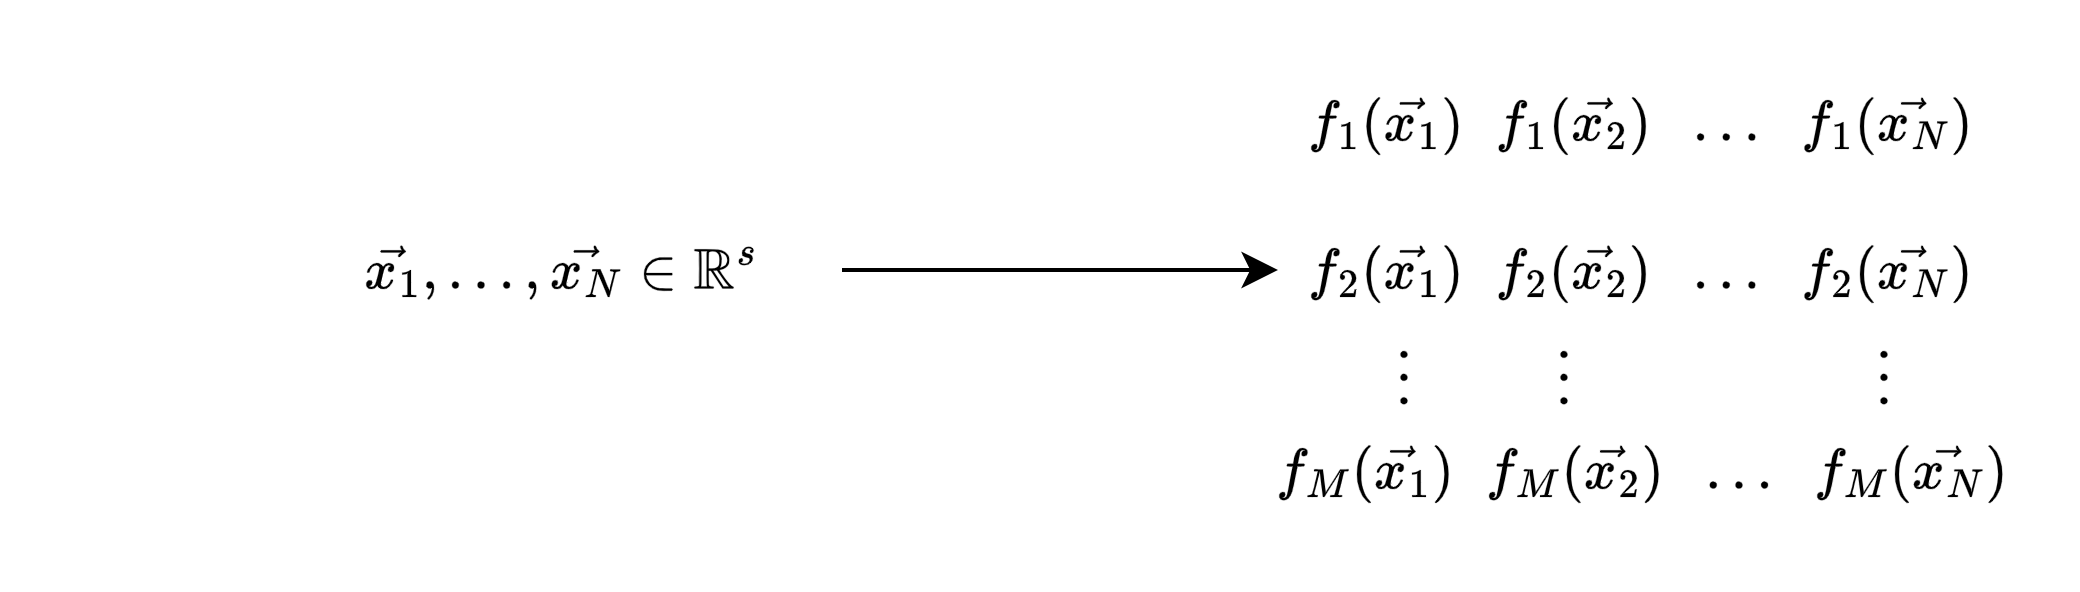
\includegraphics[width=0.8\textwidth]{matematicas/computo_capa_representacion}
    \caption{}
\end{figure}
\todo{Hacer con tikz o con draw.io. Dar una caption apropiada. Quizas en un diagrama escribir todo el proceso}
